% Options for packages loaded elsewhere
\PassOptionsToPackage{unicode}{hyperref}
\PassOptionsToPackage{hyphens}{url}
% !TeX program = pdfLaTeX
\documentclass[12pt]{article}
\usepackage{amsmath}
\usepackage{graphicx,psfrag,epsf}
\usepackage{enumerate}
\usepackage[]{natbib}
\usepackage{textcomp}


%\pdfminorversion=4
% NOTE: To produce blinded version, replace "0" with "1" below.
\newcommand{\blind}{0}

% DON'T change margins - should be 1 inch all around.
\addtolength{\oddsidemargin}{-.5in}%
\addtolength{\evensidemargin}{-1in}%
\addtolength{\textwidth}{1in}%
\addtolength{\textheight}{1.7in}%
\addtolength{\topmargin}{-1in}%

%% load any required packages here


% Pandoc syntax highlighting
\usepackage{color}
\usepackage{fancyvrb}
\newcommand{\VerbBar}{|}
\newcommand{\VERB}{\Verb[commandchars=\\\{\}]}
\DefineVerbatimEnvironment{Highlighting}{Verbatim}{commandchars=\\\{\}}
% Add ',fontsize=\small' for more characters per line
\usepackage{framed}
\definecolor{shadecolor}{RGB}{248,248,248}
\newenvironment{Shaded}{\begin{snugshade}}{\end{snugshade}}
\newcommand{\AlertTok}[1]{\textcolor[rgb]{0.94,0.16,0.16}{#1}}
\newcommand{\AnnotationTok}[1]{\textcolor[rgb]{0.56,0.35,0.01}{\textbf{\textit{#1}}}}
\newcommand{\AttributeTok}[1]{\textcolor[rgb]{0.13,0.29,0.53}{#1}}
\newcommand{\BaseNTok}[1]{\textcolor[rgb]{0.00,0.00,0.81}{#1}}
\newcommand{\BuiltInTok}[1]{#1}
\newcommand{\CharTok}[1]{\textcolor[rgb]{0.31,0.60,0.02}{#1}}
\newcommand{\CommentTok}[1]{\textcolor[rgb]{0.56,0.35,0.01}{\textit{#1}}}
\newcommand{\CommentVarTok}[1]{\textcolor[rgb]{0.56,0.35,0.01}{\textbf{\textit{#1}}}}
\newcommand{\ConstantTok}[1]{\textcolor[rgb]{0.56,0.35,0.01}{#1}}
\newcommand{\ControlFlowTok}[1]{\textcolor[rgb]{0.13,0.29,0.53}{\textbf{#1}}}
\newcommand{\DataTypeTok}[1]{\textcolor[rgb]{0.13,0.29,0.53}{#1}}
\newcommand{\DecValTok}[1]{\textcolor[rgb]{0.00,0.00,0.81}{#1}}
\newcommand{\DocumentationTok}[1]{\textcolor[rgb]{0.56,0.35,0.01}{\textbf{\textit{#1}}}}
\newcommand{\ErrorTok}[1]{\textcolor[rgb]{0.64,0.00,0.00}{\textbf{#1}}}
\newcommand{\ExtensionTok}[1]{#1}
\newcommand{\FloatTok}[1]{\textcolor[rgb]{0.00,0.00,0.81}{#1}}
\newcommand{\FunctionTok}[1]{\textcolor[rgb]{0.13,0.29,0.53}{\textbf{#1}}}
\newcommand{\ImportTok}[1]{#1}
\newcommand{\InformationTok}[1]{\textcolor[rgb]{0.56,0.35,0.01}{\textbf{\textit{#1}}}}
\newcommand{\KeywordTok}[1]{\textcolor[rgb]{0.13,0.29,0.53}{\textbf{#1}}}
\newcommand{\NormalTok}[1]{#1}
\newcommand{\OperatorTok}[1]{\textcolor[rgb]{0.81,0.36,0.00}{\textbf{#1}}}
\newcommand{\OtherTok}[1]{\textcolor[rgb]{0.56,0.35,0.01}{#1}}
\newcommand{\PreprocessorTok}[1]{\textcolor[rgb]{0.56,0.35,0.01}{\textit{#1}}}
\newcommand{\RegionMarkerTok}[1]{#1}
\newcommand{\SpecialCharTok}[1]{\textcolor[rgb]{0.81,0.36,0.00}{\textbf{#1}}}
\newcommand{\SpecialStringTok}[1]{\textcolor[rgb]{0.31,0.60,0.02}{#1}}
\newcommand{\StringTok}[1]{\textcolor[rgb]{0.31,0.60,0.02}{#1}}
\newcommand{\VariableTok}[1]{\textcolor[rgb]{0.00,0.00,0.00}{#1}}
\newcommand{\VerbatimStringTok}[1]{\textcolor[rgb]{0.31,0.60,0.02}{#1}}
\newcommand{\WarningTok}[1]{\textcolor[rgb]{0.56,0.35,0.01}{\textbf{\textit{#1}}}}

% tightlist command for lists without linebreak
\providecommand{\tightlist}{%
  \setlength{\itemsep}{0pt}\setlength{\parskip}{0pt}}



\usepackage{float}

\IfFileExists{bookmark.sty}{\usepackage{bookmark}}{\usepackage{hyperref}}
\IfFileExists{xurl.sty}{\usepackage{xurl}}{} % add URL line breaks if available
\hypersetup{
  pdftitle={Survival Analysis of Infection Control Measures in Burn Patients},
  hidelinks,
  pdfcreator={LaTeX via pandoc}}



\begin{document}


\def\spacingset#1{\renewcommand{\baselinestretch}%
{#1}\small\normalsize} \spacingset{1}


%%%%%%%%%%%%%%%%%%%%%%%%%%%%%%%%%%%%%%%%%%%%%%%%%%%%%%%%%%%%%%%%%%%%%%%%%%%%%%

\if0\blind
{
  \title{\bf Survival Analysis of Infection Control Measures in Burn
Patients}

  \author{
        Ziyue Yang \thanks{The authors gratefully acknowledge
Prof.~David Rocke and Brittany Lemmon for their instruction and guidance
throughout this project.} \\
    \\
      }
  \maketitle
} \fi

\if1\blind
{
  \bigskip
  \bigskip
  \bigskip
  \begin{center}
    {\LARGE\bf Survival Analysis of Infection Control Measures in Burn
Patients}
  \end{center}
  \medskip
} \fi

\bigskip

\noindent%
 

\vfill

\newpage
\spacingset{1.9} % DON'T change the spacing!

\section{Introduction}\label{introduction}

Infection with \emph{Staphylococcus aureus} is a critical concern in
burn patients, often contributing to prolonged hospital stays, increased
morbidity, and higher healthcare costs \citep{norbury_infection_2016}.
Therefore, effective infection control measures are of great importance.
This study investigates the impact of replacing routine bathing with
total body washing using antimicrobial agents on infection risk,
leveraging survival analysis techniques to rigorously evaluate the time
to infection. The dataset, originally published by Ichida \emph{et al.}
(1993), provides data on infection times, patient characteristics, and
clinical interventions \citep{ichida_evaluation_1993}.

To highlight differences in infection-free survival between patients
receiving routine bathing and those undergoing total body washing, the
Kaplan-Meier estimator was used \citep{kaplan_nonparametric_1958}.

To further identify factors influencing infection risk,the Cox Model was
used \citep{cox1972}. Both time-independent covariates (e.g.~patient
gender, race) and time-dependent covariates (e.g.~surgical excision of
burn tissue, prophylactic antibiotic treatment) are employed for a
comprehensive analysis of \emph{Staphylococcus aureus} infection on burn
patients.

This report aims to present a clear and actionable evaluation of the
infection control measures through the lens of survival analysis, with
insights that inform clinical decision-making and contribute to better
patient care.

\section{Results and Discussion}\label{results-and-discussion}

\subsection{Kaplan-Meier Analysis}\label{kaplan-meier-analysis}

Fig. 1 highlights differences in infection-free survival between routine
care and antimicrobial cleansing. After 30 days, 76\% of patients in the
cleansing group remained infection-free compared to 66\% in the routine
care group. By the end of the study, 70\% of cleansing patients remained
infection-free, versus 30\% in the routine care group. Nelson-Aalen
curves confirmed these trends, showing slightly higher infection-free
percentages for both groups. The survival curves do not cross,
suggesting the relative risk between the two treatment groups remains
constant over the period observed.

\begin{Shaded}
\begin{Highlighting}[]
\CommentTok{\# Plot the KM curves}
\FunctionTok{plot}\NormalTok{(KMcurves, }\AttributeTok{col =} \FunctionTok{c}\NormalTok{(}\StringTok{"black"}\NormalTok{, }\StringTok{"red"}\NormalTok{), }\AttributeTok{lwd =} \DecValTok{2}\NormalTok{, }\AttributeTok{lty =} \DecValTok{1}\NormalTok{, }\AttributeTok{xlab =} \StringTok{"Time (days)"}\NormalTok{, }\AttributeTok{ylab =} \StringTok{"Percent Infection{-}free"}\NormalTok{, }
     \AttributeTok{main =} \StringTok{"KM and NA Survival Curves for Two Types of Treatment"}\NormalTok{)}

\CommentTok{\# Add the NA curves}
\FunctionTok{lines}\NormalTok{(NAcurves, }\AttributeTok{col =} \FunctionTok{c}\NormalTok{(}\StringTok{"black"}\NormalTok{, }\StringTok{"red"}\NormalTok{), }\AttributeTok{lwd =} \DecValTok{2}\NormalTok{, }\AttributeTok{lty =} \DecValTok{2}\NormalTok{)}

\CommentTok{\# Add a legend}
\FunctionTok{legend}\NormalTok{(}\StringTok{"bottomright"}\NormalTok{, }
       \AttributeTok{legend =} \FunctionTok{c}\NormalTok{(}\StringTok{"Routine Care (KM)"}\NormalTok{, }\StringTok{"Cleansing (KM)"}\NormalTok{, }\StringTok{"Routine Care (NA)"}\NormalTok{, }\StringTok{"Cleansing (NA)"}\NormalTok{),}
       \AttributeTok{col =} \FunctionTok{c}\NormalTok{(}\StringTok{"black"}\NormalTok{, }\StringTok{"red"}\NormalTok{, }\StringTok{"black"}\NormalTok{, }\StringTok{"red"}\NormalTok{), }
       \AttributeTok{lty =} \FunctionTok{c}\NormalTok{(}\DecValTok{1}\NormalTok{, }\DecValTok{1}\NormalTok{, }\DecValTok{2}\NormalTok{, }\DecValTok{2}\NormalTok{), }
       \AttributeTok{lwd =} \DecValTok{2}\NormalTok{)}
\end{Highlighting}
\end{Shaded}

\begin{figure}
\centering
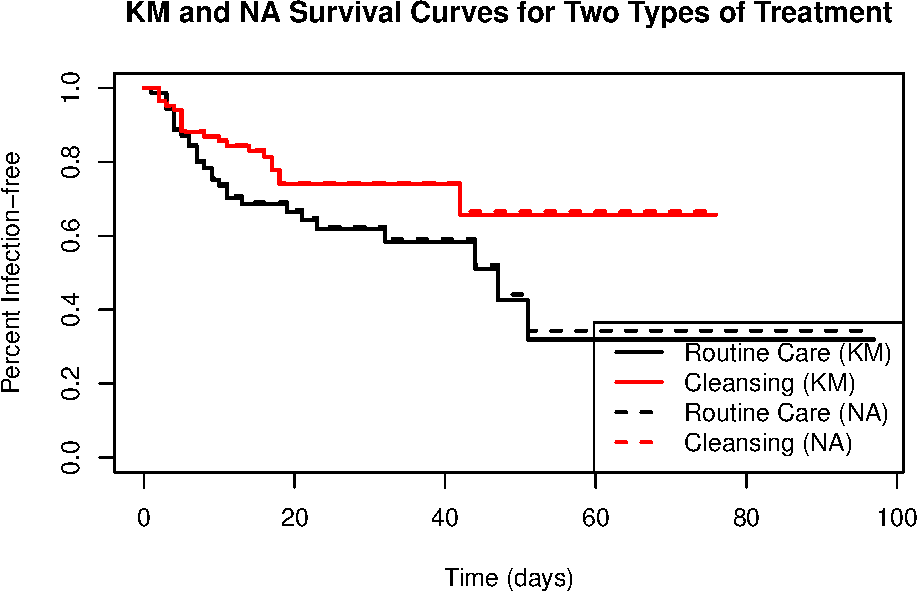
\includegraphics{Survival-Analysis-of-Infection-Control-Measures-in-Burn-Patients_files/figure-latex/fig1-1.pdf}
\caption{Fig. 1}
\end{figure}

Figure 1. Kaplan-Meier and Nelson-Aalen Survival Curves. Both KM (solid
line) and NA (dashed line) curves illustrates the proportion of patients
remaining infection-free over time for routine care (black) and
antimicrobial cleansing groups (red). Patients receiving antimicrobial
cleansing consistently showed higher infection-free survival rates
compared to routine care throughout the study.

Furthermore, The log-rank test supports this difference with
(\(\chi^2 = 3.8\), and a boarderline p-value of 0.05. Patients in the
antimicrobial cleansing group had fewer observed infections (20) than
expected (26.6), while those in the routine care group experienced more
infections (28) than expected (21.4).

These results suggest that antimicrobial cleansing offers a protective
benefit in reducing infection risks, highlighting its potential as an
effective intervention for burn patients.

\subsection{Cox Proportional Hazards
Model}\label{cox-proportional-hazards-model}

The constructed final model was determined to include Treatment, Race,
and the time-dependent covariate surgical excision, as these variables
demonstrated statistical significance and clinical relevance.

Patients who received antimicrobial cleansing were 40.4\% less likely to
develop an infection compared to those who received routine care (p =
0.082). While this result was not statistically significant in this
model, it suggests a potential protective effect of a cleansing against
\emph{Staphylococcus aureus} infection that needs to be further
validated. White patients were significantly more likely to develop an
infection compared to non-White patients, with an 8.86-fold higher
likelihood of infection (p = 0.031). The wide confidence interval (95\%
CI: 1.22--64.34) for this result reflects uncertainty, likely due to the
small sample size (n = 154). Finally, surgical excision was associated
with a 60\% lower likelihood of infection (p = 0.059), indicating a
marginal significant effect.

Overall, the cox model demonstrated good predictive performance, with a
concordance index of 0.696, meaning it correctly predicted the order of
infection risk in approximately 69.6\% of cases. The likelihood ratio
test confirmed the statistical significance of the model as a whole (p =
0.0004).

\begin{verbatim}
## Call:
## coxph(formula = burn2.surv ~ Treatment + Race + surgical, data = burn2)
## 
##   n= 288, number of events= 48 
## 
##                       coef exp(coef) se(coef)      z Pr(>|z|)  
## TreatmentCleansing -0.4843    0.6161   0.2967 -1.632   0.1026  
## RaceWhite           2.1939    8.9703   1.0117  2.169   0.0301 *
## surgical           -1.0039    0.3664   0.4834 -2.077   0.0378 *
## ---
## Signif. codes:  0 '***' 0.001 '**' 0.01 '*' 0.05 '.' 0.1 ' ' 1
## 
##                    exp(coef) exp(-coef) lower .95 upper .95
## TreatmentCleansing    0.6161     1.6230    0.3444    1.1021
## RaceWhite             8.9703     0.1115    1.2349   65.1589
## surgical              0.3664     2.7290    0.1421    0.9451
## 
## Concordance= 0.672  (se = 0.036 )
## Likelihood ratio test= 18.4  on 3 df,   p=4e-04
## Wald test            = 12.62  on 3 df,   p=0.006
## Score (logrank) test = 14.72  on 3 df,   p=0.002
\end{verbatim}

\subsection{Residual Analysis}\label{residual-analysis}

\subsubsection{Deviance Residuals}\label{deviance-residuals}

The analysis of deviance residuals revealed several cases where the
observed time to infection deviated significantly from the model's
predictions. A positive deviance residual indicates that the infection
occurred later than predicted and vice versa.

To be specific, observation 65 is a while male with 85\% percent burns
on head, buttock, trunk, upperleg, and respirtory track who received
routine care and had a deviance residual of 2.36.

Conversely, observation 15 is a white male with 20\% burns on head and
trunk, and he received routine care and no excision surgery or
antibodies. This patient had a deviance residual of -1.33, suggesting
that the observed infection occurred earlier than the model would have
predicted.

Table 1 shows the patient characteristics of high deviance residual
individuals (\textgreater2sd).

In addition to deviance residual, DEBETA values were computed to measure
influential observations. Large DFBETA values indicate that a specific
observation has a strong effect on a particular predictor and may need
further investigation.

For example, observation 91 is a white male with 20\% burns, and he
received cleansing care with both excision surgery and antibiotic
treatment. This patient has a large influence on the time-dependent
covariate coefficient \texttt{surgery} with a DFBETA value = 0.137.
Additionally, observation 92 is a white male with 5\% burns, and he
received cleansing care and excision surgery. This observation also has
a large influence on the coefficient of \texttt{surgery} with a DEBETA
value = 0.212. Interestingly, he also has a high deviance residual
value.

Table 1 shows the characistics of patients with a high DFBETA value.

Since this is an association study instead of causal study so we failed
to consider the confounder relationship and matching. We spend more
effort on statical meaning for the prediction based on AIC based on
their burn situation and demographics.

\section{Conclusion}\label{conclusion}

In conclusion, the risk of infection was 40.4\% lower in patients who
received cleansing care, although not statistically significant. There
was also some indication that excision surgery may be important for
infection control.

\section{Appendices}\label{appendices}

\section{Data Description}\label{data-description}

The dataset \texttt{burn} consists of 154 observations of burn patients
and 17 variables that capture patient characteristics, clinical
interventions, and infection status with time to infection.

\subsection{\texorpdfstring{\textbf{Outcome
Variables}}{Outcome Variables}}\label{outcome-variables}

\begin{itemize}
\tightlist
\item
  \textbf{T3 (time to infection)}: The time (in days) until infection
  with \emph{Staphylococcus aureus}.
\item
  \textbf{D3 (infection status)}: A binary variable indicating whether
  the patient developed an infection within the course of the study (1 =
  infected, 0 = not infected).
\end{itemize}

\subsection{\texorpdfstring{\textbf{Time-Dependent
Covariates}}{Time-Dependent Covariates}}\label{time-dependent-covariates}

\begin{itemize}
\tightlist
\item
  \textbf{T1 (time to surgical excision)}: The time (in days) to
  surgical excision of burn tissue.
\item
  \textbf{D1 (surgical excision status)}: A binary variable indicating
  whether surgical excision was performed (1 = excised, 0 = not
  excised).
\item
  \textbf{T2 (time to antibiotic treatment)}: The time (in days) to the
  administration of prophylactic antibiotic treatment.
\item
  \textbf{D2 (antibiotic treatment status)}: A binary variable
  indicating whether antibiotics were administered (1 = treated, 0 = not
  treated).
\end{itemize}

\subsection{\texorpdfstring{\textbf{Baseline
Characteristics}}{Baseline Characteristics}}\label{baseline-characteristics}

\begin{itemize}
\tightlist
\item
  \textbf{Treatment}: Categorical variable indicating the bathing
  regimen (Routine or Cleansing with antimicrobial agents).
\item
  \textbf{Gender}: Categorical variable indicating the patient's gender
  (Male or Female).
\item
  \textbf{Race}: Categorical variable indicating the patient's race
  (Nonwhite or White).
\item
  \textbf{PercentBurned}: Numeric variable representing the percentage
  of the patient's body surface area affected by burns.
\end{itemize}

\subsection{\texorpdfstring{\textbf{Burn Site
Characteristics}}{Burn Site Characteristics}}\label{burn-site-characteristics}

\begin{itemize}
\tightlist
\item
  \textbf{SiteHead}: Binary factor indicating whether the head was
  burned (Burned or Not Burned).
\item
  \textbf{SiteButtock}: Binary factor indicating whether the buttocks
  were burned (Burned or Not Burned).
\item
  \textbf{SiteTrunk}: Binary factor indicating whether the trunk was
  burned (Burned or Not Burned).
\item
  \textbf{SiteUpperLeg}: Binary factor indicating whether the upper leg
  was burned (Burned or Not Burned).
\item
  \textbf{SiteLowerLeg}: Binary factor indicating whether the lower leg
  was burned (Burned or Not Burned).
\item
  \textbf{SiteRespTract}: Binary factor indicating whether the
  respiratory tract was burned (Burned or Not Burned).
\end{itemize}

\subsection{\texorpdfstring{\textbf{Burn
Type}}{Burn Type}}\label{burn-type}

\begin{itemize}
\tightlist
\item
  \textbf{BurnType}: Categorical variable specifying the type of burn
  (Chemical, Scald, Flame, or Electric).
\end{itemize}

\section{Methods}\label{methods}

\subsection{\texorpdfstring{\textbf{Kaplan-Meier Survival
Analysis}}{Kaplan-Meier Survival Analysis}}\label{kaplan-meier-survival-analysis}

\begin{verbatim}
## Call:
## survdiff(formula = burn1.surv ~ Treatment, data = burn1)
## 
##                      N Observed Expected (O-E)^2/E (O-E)^2/V
## Treatment=Routine   70       28     21.4      2.07      3.79
## Treatment=Cleansing 84       20     26.6      1.66      3.79
## 
##  Chisq= 3.8  on 1 degrees of freedom, p= 0.05
\end{verbatim}

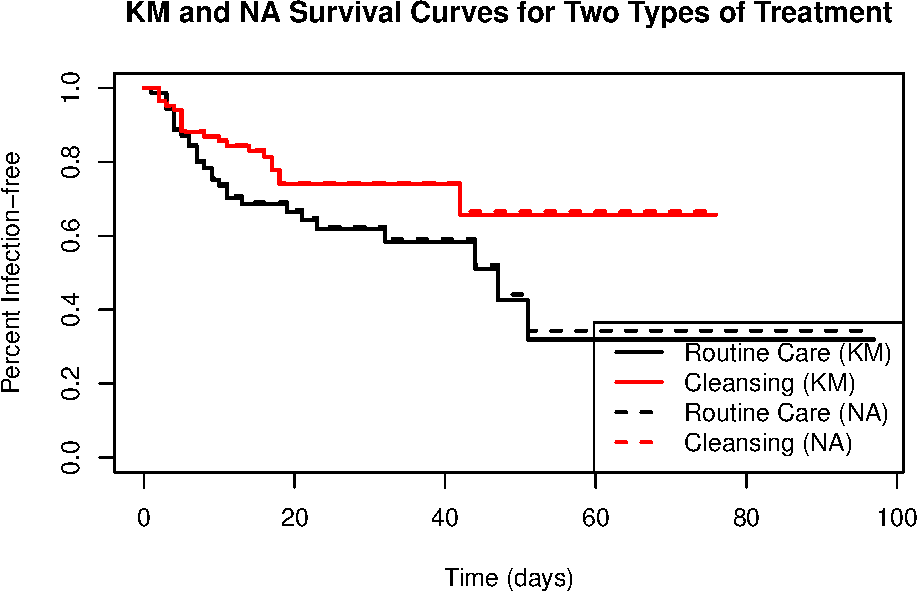
\includegraphics{Survival-Analysis-of-Infection-Control-Measures-in-Burn-Patients_files/figure-latex/unnamed-chunk-6-1.pdf}
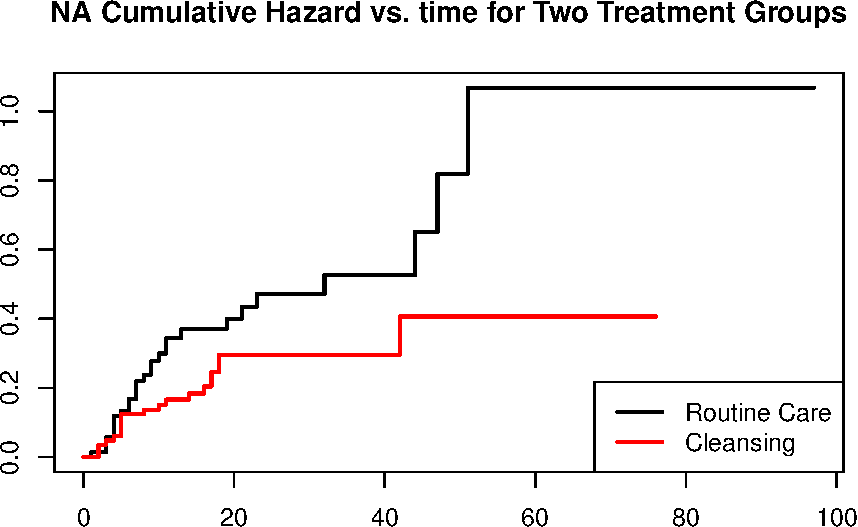
\includegraphics{Survival-Analysis-of-Infection-Control-Measures-in-Burn-Patients_files/figure-latex/unnamed-chunk-6-2.pdf}
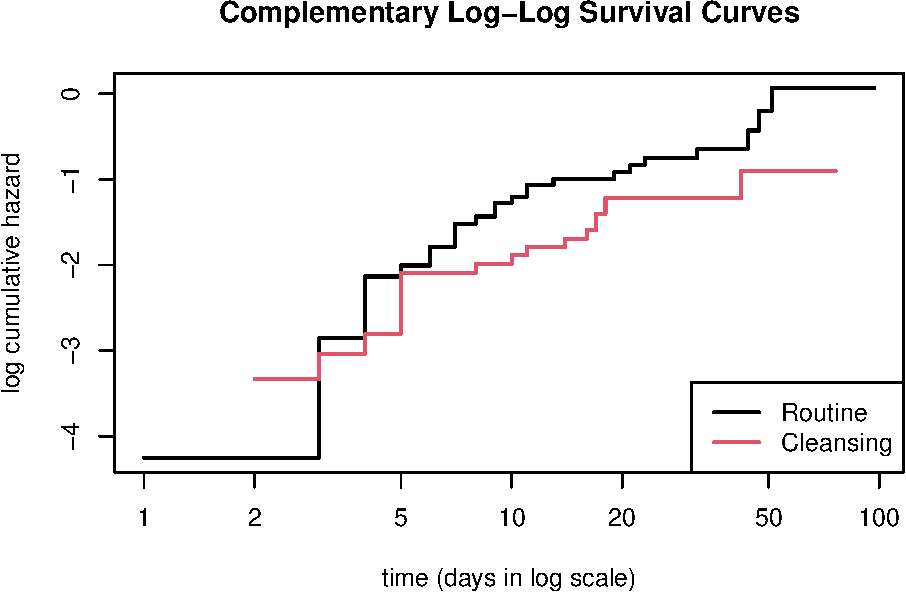
\includegraphics{Survival-Analysis-of-Infection-Control-Measures-in-Burn-Patients_files/figure-latex/unnamed-chunk-6-3.pdf}

The Kaplan-Meier estimator was used to estimate and visualize the
probability of remaining infection-free over time for patients
undergoing either routine bathing or antimicrobial washing.
Additionally, Nelson-Aalen estimate was also plotted for a comprehensive
view of survival difference between groups.

Survival curves were compared using the \texttt{survdiff} function in
package \texttt{survival}, which performs a log-rank test to assess
whether the differences between the two groups are statistically
significant.

Additionally, cumulative hazard functions were plotted against time to
estimate the cumulative infection probability at different time points.
Complementary log-log survival curves were plotted against
log-transformed time to assess if the ratio of hazard rates between two
treatment groups remains constant over time.

\subsection{\texorpdfstring{\textbf{Cox Proportional Hazards
Model}}{Cox Proportional Hazards Model}}\label{cox-proportional-hazards-model-1}

\subsubsection{\texorpdfstring{\textbf{Model with Time-Independent
Covariates}}{Model with Time-Independent Covariates}}\label{model-with-time-independent-covariates}

An initial Cox proportional hazards model was constructed using
time-independent covariates to evaluate their relationship with the risk
of infection. The primary predictor of interest was \textbf{Treatment}.
Additional time-independent variables were sequentially introduced into
the model.

To address the violation of the proportional hazards assumption
identified in the unstratified model, the variable
\textbf{SiteRespTract} was stratified. This allowed for differing
baseline hazard functions for patients with and without burns in the
respiratory tract.

Model refinement was performed using the \texttt{drop1} function to
identify covariates that did not significantly contribute to model
performance. Multicollinearity among covariates was assessed using
variance inflation factors, ensuring that redundant predictors were
identified and addressed without compromising the integrity of the
model.

\subsubsection{\texorpdfstring{\textbf{Model with Time-Dependent
Covariates}}{Model with Time-Dependent Covariates}}\label{model-with-time-dependent-covariates}

To incorporate time-dependent predictors, the dataset was expanded using
counting process notation. Two key time-dependent covariates were
included: 1. \textbf{Surgical excision of burn tissue (T1, D1)}. 2.
\textbf{Prophylactic antibiotic treatment (T2, D2)}.

A Cox model was constructed combining time-dependent and
time-independent covariates. The time-dependent variables captured the
dynamic effects of these interventions on infection risk, while
time-independent variables provided baseline hazard adjustments.

\subsection{\texorpdfstring{\textbf{Model Checking and
Diagnostics}}{Model Checking and Diagnostics}}\label{model-checking-and-diagnostics}

Model checking was performed using a comprehensive suite of diagnostic
techniques:

\subsubsection{\texorpdfstring{\textbf{Proportional Hazards
Assumption}}{Proportional Hazards Assumption}}\label{proportional-hazards-assumption}

The proportional hazards assumption was evaluated using Schoenfeld
residual plots which test whether the residuals show systematic trends
over time and \texttt{cox.zph} function from package \texttt{survival}.
Where violations were detected, appropriate adjustments were made, such
as stratification to allow baseline hazard functions to differ between
groups.

\subsubsection{\texorpdfstring{\textbf{Goodness-of-Fit}}{Goodness-of-Fit}}\label{goodness-of-fit}

Cox-Snell residuals were used to assess overall model fit. A cumulative
hazard plot was constructed to compare observed data with the expected
hazard under the model. A straight 45-degree line indicated good fit,
while deviations suggested potential inadequacies.

\subsubsection{\texorpdfstring{\textbf{Outlier
Analysis}}{Outlier Analysis}}\label{outlier-analysis}

Residual analysis was performed to evaluate how well the Cox model
aligned with the observed data and to identify unusual observations. Two
types of residuals -- deviance residuals and DFBETA values -- were
analyzed.

Deviance residuals are derived from martingale residuals and measure how
much an individual's observed time to infection deviates from the
model's prediction, with positive values indicating later-than-expected
infections.

DFBETA values measure the influence of individual observations on the
model's coefficients. Large DFBETA values indicate that a specific
observation has a strong effect on a particular predictor.

Using thresholds based on two standard deviations from the mean for each
residual type, observations were flagged as unusual.

\begin{Shaded}
\begin{Highlighting}[]
\FunctionTok{library}\NormalTok{(knitr)}

\CommentTok{\# Add deviance residuals to the burn2 dataset}
\NormalTok{burn2}\SpecialCharTok{$}\NormalTok{Deviance }\OtherTok{\textless{}{-}}\NormalTok{ deviance\_residuals}

\CommentTok{\# Define the threshold for extreme deviance residuals (e.g., absolute value \textgreater{} 2)}
\NormalTok{threshold }\OtherTok{\textless{}{-}} \DecValTok{2}

\CommentTok{\# Filter patients with extreme deviance residuals}
\NormalTok{extreme\_table }\OtherTok{\textless{}{-}}\NormalTok{ burn2[}\FunctionTok{abs}\NormalTok{(burn2}\SpecialCharTok{$}\NormalTok{Deviance) }\SpecialCharTok{\textgreater{}}\NormalTok{ threshold, ]}

\CommentTok{\# Select relevant columns including surgical and antibiotic care}
\NormalTok{extreme\_table }\OtherTok{\textless{}{-}}\NormalTok{ extreme\_table[, }\FunctionTok{c}\NormalTok{(}\StringTok{"Obs"}\NormalTok{, }\StringTok{"Gender"}\NormalTok{, }\StringTok{"Race"}\NormalTok{, }\StringTok{"PercentBurned"}\NormalTok{, }
                                   \StringTok{"Treatment"}\NormalTok{, }\StringTok{"surgical"}\NormalTok{, }\StringTok{"antibiotics"}\NormalTok{, }\StringTok{"Deviance"}\NormalTok{)]}
\end{Highlighting}
\end{Shaded}

\begin{Shaded}
\begin{Highlighting}[]
\FunctionTok{kable}\NormalTok{(extreme\_table, }
      \AttributeTok{caption =} \StringTok{"Table 1: Patient Characteristics with Extreme Deviance Residuals"}\NormalTok{,}
      \AttributeTok{col.names =} \FunctionTok{c}\NormalTok{(}\StringTok{"Observation"}\NormalTok{, }\StringTok{"Gender"}\NormalTok{, }\StringTok{"Race"}\NormalTok{, }\StringTok{"Burn Percentage"}\NormalTok{, }
                    \StringTok{"Treatment Type"}\NormalTok{, }\StringTok{"Surgical Care"}\NormalTok{, }\StringTok{"Antibiotic Care"}\NormalTok{, }\StringTok{"Deviance Residual"}\NormalTok{),}
      \AttributeTok{align =} \StringTok{"c"}\NormalTok{)}
\end{Highlighting}
\end{Shaded}


\bibliographystyle{plain}
\bibliography{bibliography.bib}



\end{document}
